\documentclass{beamer}

\usetheme{default}
\usecolortheme{rose}
\usepackage{hyperref}
\usepackage{array}
\newcommand{\ignore}[1]{}
\newcommand{\pr}{\mathbb{P}}
\newcommand{\E}{\mathbb{E}}
\newcommand{\Var}{\text{var}}
\newcommand{\SD}{\text{sd}}
\setbeamerfont{alerted text}{series=\itshape}
\addtobeamertemplate{navigation symbols}{}{%
    \usebeamerfont{footline}%
    \usebeamercolor[fg]{footline}%
    \hspace{1em}%
    \insertframenumber/\inserttotalframenumber
}

\newcolumntype{P}[1]{>{\centering\arraybackslash}p{#1}}

\title{Random Variables}

% A subtitle is optional and this may be deleted
\subtitle{STAT-UB.0001 Statistics for Business Control}

\author{Ningshan Zhang}
% - Give the names in the same order as the appear in the paper.
% - Use the \inst{?} command only if the authors have different
%   affiliation.

\institute[New York University] % (optional, but mostly needed)
{
  IOMS Department\\
  nzhang@stern.nyu.edu
  \let\thefootnote\relax\footnotetext{\tiny{*  Office Hours: Wed \& Fri 10:00 - 11:30 AM, KMC 8-174}}
}
\date{Jul 12, 2018}
\AtBeginSubsection[]
{
  \begin{frame}<beamer>{Outline}
    \tableofcontents[currentsection,currentsubsection]
  \end{frame}
}

% Let's get started
\begin{document}

%-------------------
\begin{frame}
  \titlepage
\end{frame}



% Section and subsections will appear in the presentation overview
% and table of contents.
%-------------------
\begin{frame}{Review}
\begin{itemize}
\item Independence, Bayes' Rule
\item Counting: Permutations, Combinations
\end{itemize}
\end{frame}

%-------------------
\begin{frame}{Random Variable}
    \begin{block}{Random Variable}
        A variable whose value depends uniquely on the outcome of a random experiment. 
        Usually denoted by capital letters, e.g. $X,Y,Z$.
    \end{block}

\vspace{\stretch{0.5}}
    More interpretations:
\begin{itemize}
%\item A random variable refers to the result of a random experiment.
\item A random variable maps sample points of a random experiment to values. 
\item Once the experiment is performed, the value of the random variable is referred to as an \alert{observation}. 
\item A data set contains observations of a random variable resulting from repeated trials of the random experiment.
\end{itemize}
\end{frame}


%-------------------
\begin{frame}{Random Variable: More Examples}
\begin{itemize}
\item Example 1
\begin{itemize}
\item Random experiment: Roll two dices.
\item $X = \text{ sum of the two dices}$.
\item Observe $2$ and $4$ from one trial of the experiment, $X=6$.
\end{itemize}
\vspace{\stretch{0.5}}
\item Example 2
\begin{itemize}
\item Random experiment: flip a coin three times.
\item $X = \text{ number of heads from the three flips}$.
\item Observe HHT from one trial of the experiment, $X=2$.
\end{itemize}
\end{itemize}
\end{frame}

%-------------------
\begin{frame}{Two Types of Random Variables}
\begin{block}{Discrete random variable}
Can take a countable (finite or infinite) number of values, often obtained from ``counting''.
\end{block}
Example: Number of heads when flipping three coins.

\vspace{\stretch{0.5}}
\begin{block}{Continuous random variable}
Can take any value in an interval of real numbers.
Uncountable.  Often obtained from ``measuring''.
\end{block}
Example: Average height of 3 students randomly picked from this class.
\end{frame}

%-------------------
\begin{frame}{Case Study}
Consider the following game:
\begin{enumerate}
\item You pay \$6 to flip a coin.
\item If the coin lands heads, you get \$10; otherwise, you get nothing.
\end{enumerate}

\vspace{\stretch{0.5}}
Let $W$ be the random variable equal to the amount of money you win (can be negative).
\vspace{\stretch{0.2}}
\begin{center}
\begin{tabular}{|P{2.5cm}|P{2cm}|P{2cm}|} \hline
Sample point & $W$ & Probability\\ \hline
H &  & \\ \hline
T & &  \\ \hline
\end{tabular}
\end{center}
\end{frame}

%-------------------
\begin{frame}{Probability Distribution Function (PDF) for Discrete RV}

\begin{block}{Probability Distribution Function (PDF)}
For a discrete random variable $X$, we denote the probability that \alert{$X$} takes the value \alert{$x$} by
$$ p(x) = \pr(X=x).$$

$p(x)$ is referred to as the \alert{probability distribution function} (PDF) of random variable $X$.
\end{block}

\vspace{\stretch{0.5}}
\begin{itemize}
\item A PDF can be described with a table listing every possible values of random variable, and the probability of each value.
\item In the previous case study, what is the PDF of $W$? 
\end{itemize}
\end{frame}


%-------------------
\begin{frame}{Notations for RV and its Values}
\begin{itemize}
\item Use capital letters (e.g. $X$, $W$) for the random variable.
\item Use lower case letters (e.g. $x$, $w$) for any particular value that you are interested in.
\end{itemize}

\vspace{\stretch{0.2}}
The PDF $p(x)$ is the probability of \alert{$X$} takes the value of \alert{$x$}. 
\end{frame}

%-------------------
\begin{frame}{PDF}
Sometimes it's useful to look at a graphical representation of the PDF.

\begin{figure}
    \caption{PDF for $X=\text{number of heads in three coin flips}$.}
    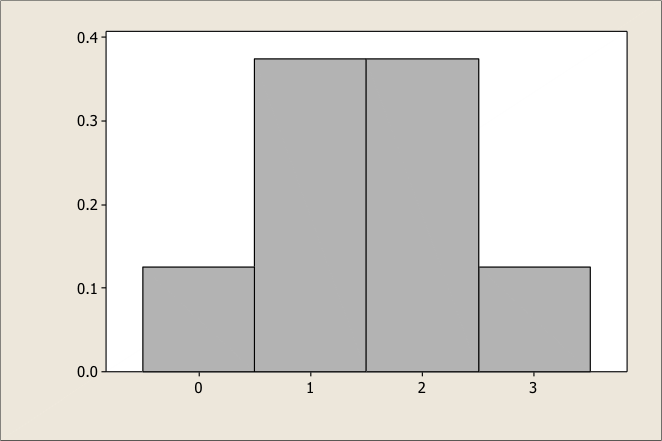
\includegraphics[width=0.6\textwidth]{figures/PDF.png}
\end{figure}

\let\thefootnote\relax\footnotetext{\tiny{* Total shaded area is 1.}}
\end{frame}

%-------------------
\begin{frame}{Expected Value}
\begin{block}{Expected value}
The expected value (or mean, expectation) of a discrete random variable $X$ is
$$\E(X)=\sum_{x} x\cdot p(x)$$
Sometimes write $\mu$, or $\mu_X$.
\end{block}

\vspace{\stretch{0.5}}
\begin{itemize}
\item $\E(X)$ can be interpreted as the long run average of $X$.
\item $\E(X)$ is not informative to predict a single run of the experiment.
\item The sample mean $\bar x$ is an estimate for $\E(X)$.
\end{itemize}
\end{frame}

%-------------------
\begin{frame}{Variance and Standard Deviation}
\begin{block}{Variance}
The variance of a discrete random variable $X$ is 
$$ \Var(X) = \sum_x (x-\mu)^2 p(x) $$
Also write $\sigma^2$, or $\sigma_X^2$.
\end{block}

\vspace{\stretch{0.5}}
To compute the variance of a discrete random variable $X$:
\begin{enumerate}
\item Compute $\mu=\E(X)$.
\item For each possible $x$, compute $(x – \mu)^2 p(x)$.
\item Add up these values.
\end{enumerate}

\ignore{
\vspace{\stretch{0.5}}
The standard deviation of $X$ is $\SD(X)=\sqrt{\Var(X)}$. Also write $\sigma$, or $\sigma_X$.
}
\end{frame}


%-------------------
\begin{frame}{Variance and Standard Deviation}
\begin{block}{Standard deviation}
The standard deviation (SD) of $X$ is 
$$\SD(X)=\sqrt{\Var(X)} = \sqrt{\sum_x (x-\mu)^2 p(x) }$$ 
Also write $\sigma$, or $\sigma_X$.
\end{block}
\end{frame}

%-------------------
\begin{frame}{Variance and Standard Deviation}
Interpretation of $\Var(X)$:
\begin{itemize}
\item The expected value of $(X-\mu)^2$: $$\Var(X)=\E\Big[(X-\mu)^2\Big]$$
\item Long run average squared deviation from the mean.
\item The sample variance $s^2$ is an estimate for $\sigma^2$.
\end{itemize}
\end{frame}


%-------------------
\begin{frame}{Empirical Rule}
If the probability distribution is bell-shaped, then,
\begin{align*}
& \pr(\mu -\sigma  <X< \mu + \sigma)  \approx 0.68 \\
& \pr(\mu -2\sigma <X< \mu +2\sigma)  \approx 0.95 \\
& \pr(\mu -3\sigma <X< \mu +3\sigma)  \approx 0.997
\end{align*}
\end{frame}


%-------------------
\begin{frame}{Properties of Expected Value}
%\begin{block}{The affine transformation property}
%Let $a,b$ be two constants, and let $X$ be a random variable. Then,
%$$ \E(aX+b) = a \E(X) + b$$
%\end{block}
%Example: measure the room temprature in Fahrenheit. Convert to Celcius: $C=(F-32)*5/9$.
%
%\begin{block}{The sum property}
%Let $X$ and $Y$ be two random variables. Then,
%$$ \E(X+Y) = \E(X)+\E(Y)$$
%\end{block}
%Example: 

\begin{enumerate}
\item (Aaffine transformation) Let $a,b$ be two constants, and let $X$ be a random variable. Then,
$$ \E(aX+b) = a \E(X) + b$$
\vspace{-0.4cm}
\begin{itemize}
\item Example: Measure the room temprature in Fahrenheit and convert to Celcius ($C=(F-32)/1.8$).
\end{itemize}
\item (Sum) Let $X$ and $Y$ be two random variables. Then,
$$ \E(X+Y) = \E(X)+\E(Y)$$
\vspace{-0.4cm}
\begin{itemize}
\item Example: Count number of male and female students in the class, and compute total number of students in the class.
\end{itemize}
\end{enumerate}
\end{frame}


%-------------------
\begin{frame}{Summary}
Random Variable
\begin{itemize}
\item Probability distribution function (PDF)
\item Expected value of a random variable
\item Variance and standard deviation of a random variable
\item Properties of expected value
\end{itemize}
\end{frame}
\ignore{
%-------------------
\begin{frame}{Time Series Plot}
\begin{figure}
    \caption{}
    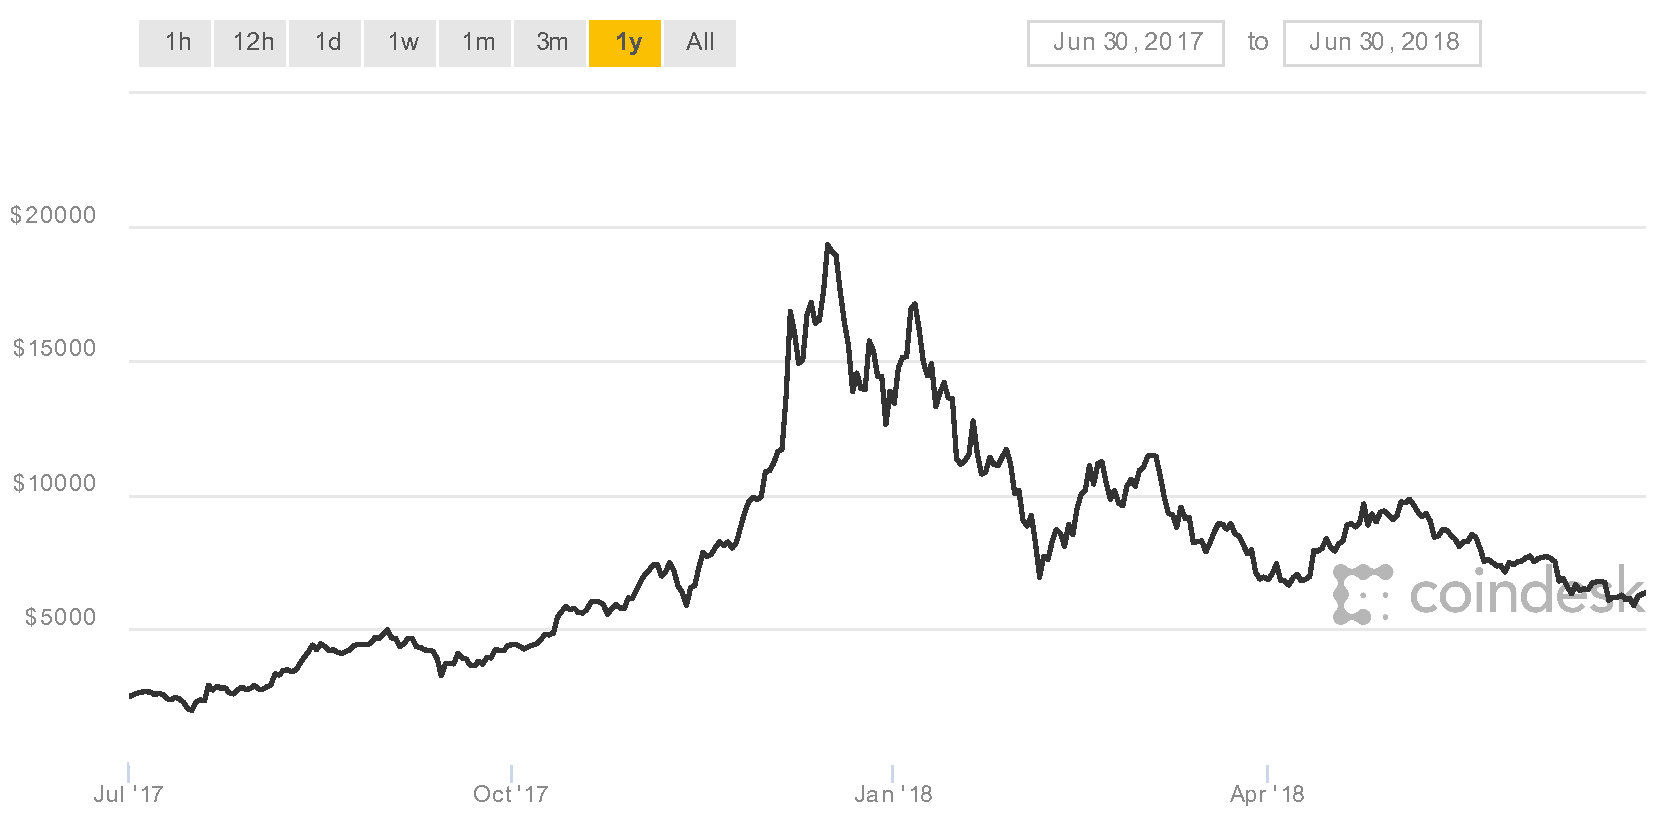
\includegraphics[width=1\textwidth]{figures/coindesk-bpi-chart}
\end{figure}
\let\thefootnote\relax\footnotetext{\tiny{* Plot from Coindesk.com}}
\end{frame}

\begin{frame}{}
\begin{itemize}
\item 
\end{itemize}
\end{frame}

\vspace{\stretch{0.5}}

\begin{block}{}
\end{block}


}

\end{document}


